\documentclass[conference]{IEEEtran}
\IEEEoverridecommandlockouts

\usepackage{cite}
\usepackage{amsmath,amssymb,amsfonts}
\usepackage{algorithmic}
\usepackage{graphicx}
\graphicspath{{figures/}}
\usepackage{textcomp}
\usepackage{xcolor}
\usepackage{booktabs}
\usepackage{url}
\usepackage{hyperref}
\usepackage{inputenc}
\usepackage[T1]{fontenc}

\def\BibTeX{{\rm B\kern-.05em{\sc i\kern-.025em b}\kern-.08em
    T\kern-.1667em\lower.7ex\hbox{E}\kern-.125emX}}

\begin{document}

\title{Cross-Layer Video Delivery over Open OFDM-ISAC:\\
Measuring Container Fragility and Outer-Code Sufficiency}

\author{
  \IEEEauthorblockN{Jiarui Ye}
  \IEEEauthorblockA{
    \textit{Shanghai Maritime University}\\
    Shanghai, China\\
    \textit{[email to be added]}
  }
}

\maketitle

\begin{abstract}
Real-time video delivery over integrated sensing and communication (ISAC) links faces a qualitatively different challenge from file transfer: residual bit errors that survive forward error correction propagate through inter-frame prediction and are amplified by the encapsulation layer before the decoder ever sees them. This paper presents the first systematic measurement of these two amplification mechanisms on a live OFDM-ISAC platform. Using OpenISAC with USRP N320 and B210 software-defined radios over an indoor over-the-air link, we (i)~conduct a Pareto scan of four Reed-Solomon outer codes and show that the LDPC(1008,504) residual error rate is below $5\times10^{-10}$, making the lightest RS(255,223) configuration both necessary and sufficient---recovering 8.4\% payload throughput over the deployed heavier code with zero steady-state block failures; and (ii)~model and directly measure the MPEG transport stream container amplification factor~$\gamma$, deriving $\gamma\approx 7$ from a Markov-chain header-exposure model and measuring $\gamma=4$--$500$ across three decoder stacks. Replacing MPEG-TS with bare H.264 Annex~B and tuning queue depths to non-blocking minima yielded $250\,\text{ms} \pm 0.5\,\text{ms}$ end-to-end latency---of which the ISAC radio contributes only $\approx\!3\,\text{ms}$---with zero-error payload delivery and $2.5\times$ throughput headroom. These results reveal that on a strongly coded ISAC link, the container and decoder layer dominates video quality far more than the outer FEC code.
\end{abstract}

\begin{IEEEkeywords}
ISAC, OFDM, real-time video, MPEG-TS, Reed-Solomon, LDPC, cross-layer design, software-defined radio
\end{IEEEkeywords}

% ─────────────────────────────────────────────────────────────────────────────
\section{Introduction}
\label{sec:intro}

Integrated sensing and communication (ISAC) is a key enabler for 6G networks, sharing waveforms, hardware, and spectrum between data transmission and environmental radar sensing~\cite{itu2023,liu2022isac,wei2023survey}. Open platforms such as OpenISAC~\cite{zhou2026openisac} now allow complete physical-layer experimentation over the air, making live ISAC links accessible to the research community with commodity USRP hardware.

Real-time video is among the most demanding payloads an ISAC link can carry. Unlike file transfer---where ARQ repairs residual FEC errors silently---inter-frame codecs such as H.264/AVC propagate damage across an entire group of pictures (GOP) from a single corrupted macroblock~\cite{wiegand2003h264}. The video service therefore couples the sparse error statistics of a strongly coded OFDM physical layer to design decisions at the container, decoder, and buffer layers that existing ISAC experimental studies leave unexamined: prior work targets sensing estimation accuracy or raw link throughput~\cite{zhou2026openisac,brunner2024bistatic}, not a running media service.

This paper closes that gap with three contributions, all derived from controlled over-the-air experiments without new hardware:
\begin{enumerate}
  \item \textbf{RS outer-code Pareto analysis.} We show empirically that the LDPC(1008,504) inner code's residual BER on a QPSK indoor link is below $5\times10^{-10}$, that all four tested RS(255,$K$) configurations achieve zero steady-state failures, and that the lightest (RS(255,223), 14.3\% redundancy) is therefore Pareto-optimal, recovering 8.4\% payload throughput over the deployed RS(255,191).

  \item \textbf{MPEG-TS container fragility: model and measurement.} We derive a Markov-chain model of TS parser behavior under residual errors, predicting a header-exposure amplification factor $\gamma\approx 7$, and measure $\gamma=4$--$500$ empirically across three decoder stacks under a controlled stress test. To our knowledge, this is the first measurement of $\gamma$ on a live ISAC platform.

  \item \textbf{Latency optimization.} We identify and eliminate a positive-feedback latency accumulation loop; the resulting service pins at $250\,\text{ms}\pm0.5\,\text{ms}$ end-to-end, with $\approx\!80\%$ attributed to the H.264 decoder and only $\approx\!3\,\text{ms}$ to the ISAC radio.
\end{enumerate}

These results support a \emph{least-sufficient protection} design rule: on a strongly coded ISAC link, outer FEC redundancy should be sized to the measured residual, and the budget freed by that reduction should be reinvested at the container and decoder layer, where protection is genuinely scarce.

% ─────────────────────────────────────────────────────────────────────────────
\section{System Description}
\label{sec:system}

\subsection{Platform}

All experiments use OpenISAC~\cite{zhou2026openisac}, an open-source C++ OFDM-ISAC platform on USRP hardware. The base station (BS) uses a NI~USRP~N320 (dual-channel, 200\,MHz FPGA, GPSDO-disciplined clock) connected over SFP$+$ 10\,GbE; the user equipment (UE) uses a NI~USRP~B210 (AD9361 front end, USB~3.0). Both sides use log-periodic antennas (6--8\,dBi). OpenISAC's resource model supports explicit \texttt{payload} and \texttt{sensing\_pilot} resource-block types within each OFDM frame, allowing communication and sensing to share the waveform with configurable resource separation; both functions run concurrently in all experiments (Fig.~\ref{fig:topology}).

\begin{figure}[t]
  \centering
  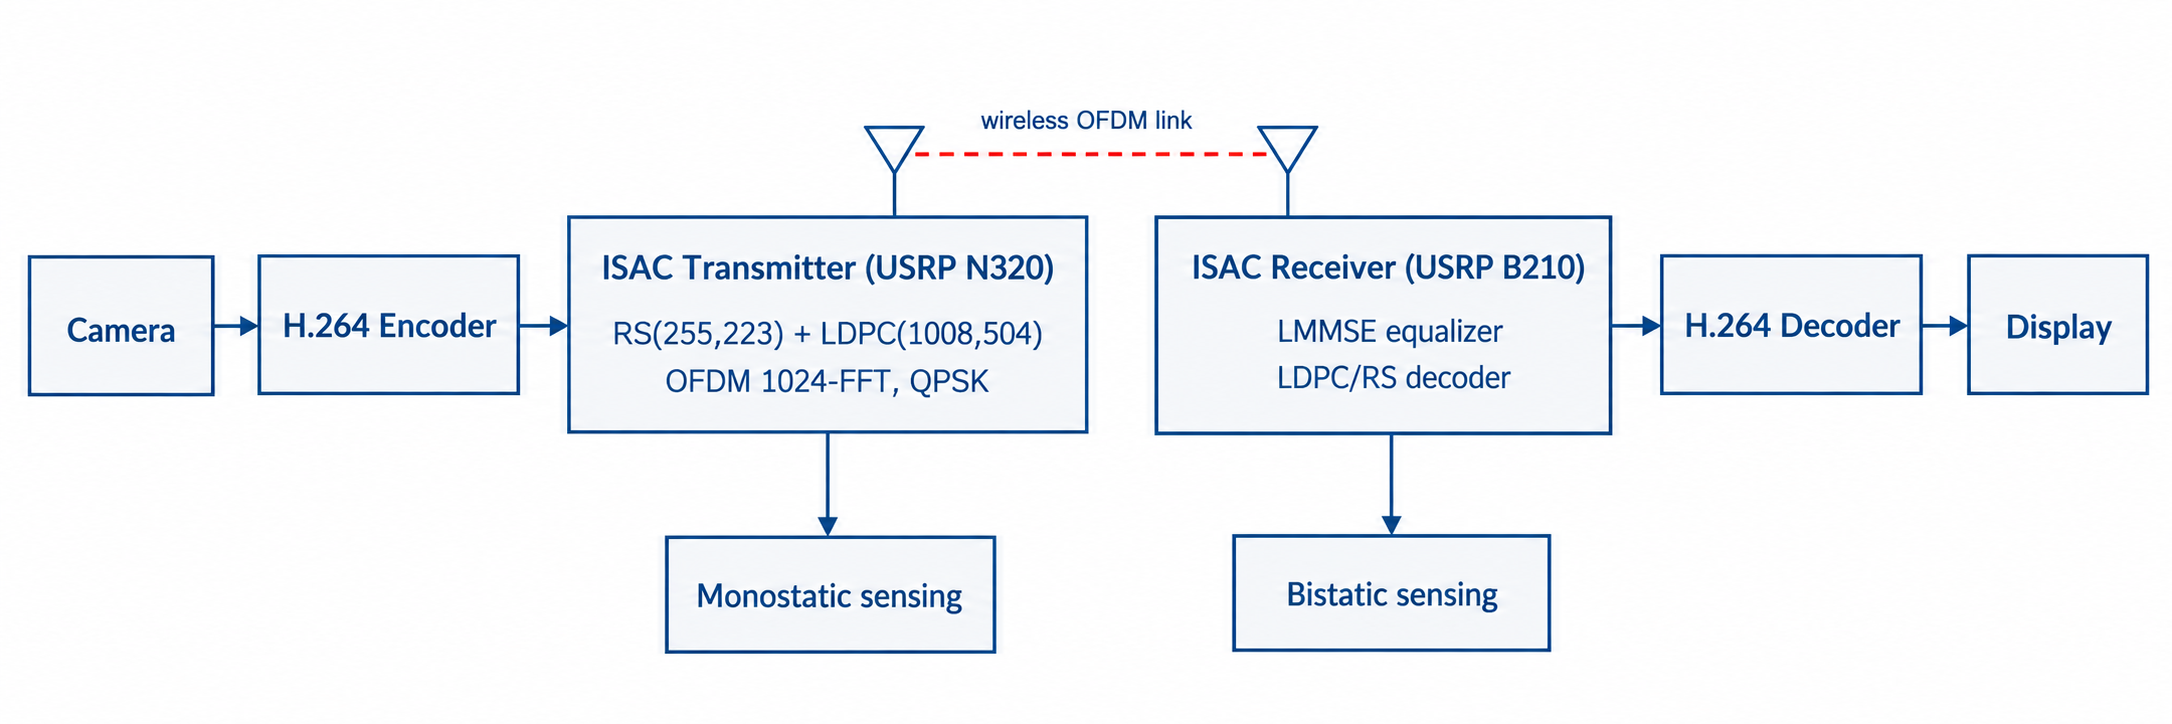
\includegraphics[width=\columnwidth]{fig1_topology.png}
  \caption{System topology. Real-time video service on the OpenISAC platform: camera $\to$ H.264 encoder $\to$ ISAC transmit chain (RS--LDPC concatenated coding over OFDM) $\to$ wireless link $\to$ ISAC receive chain $\to$ H.264 decoder $\to$ display. Payload and sensing\_pilot resource blocks share the OFDM frame; sensing runs concurrently.}
  \label{fig:topology}
\end{figure}

The video pipeline is:
\begin{equation*}
\text{camera} \to \text{x264} \to \underbrace{\text{ISAC TX (N320)}}_{\text{RS+LDPC+OFDM}} \xrightarrow{\text{air}} \underbrace{\text{ISAC RX (B210)}}_{\text{OFDM+LDPC+RS}} \to \text{decoder}
\end{equation*}

\subsection{OFDM Waveform}

The frame uses FFT size $N=1024$, cyclic prefix $G=128$ (2.56\,$\mu$s, 12.5\% overhead), 100 symbols per frame, and a 50\,MHz sampling rate, giving a frame duration of 2.304\,ms ($\approx\!434$\,frames/s) and a subcarrier spacing of 48.828\,kHz. Symbol~1 carries a Zadoff--Chu synchronization sequence (root $u=29$). Eight uniformly spaced pilot subcarriers support LMMSE channel estimation, CFO/SFO tracking, and zero-forcing equalization; reducing from 16 to 8 pilots released 792 additional resource elements per frame with no measurable channel estimation degradation.

\subsection{Concatenated Coding Chain}

\begin{equation*}
\underbrace{\text{UDP}}_{\text{payload}} \to \underbrace{\text{RS}(255,K)}_{\text{outer}} \to \underbrace{\text{LDPC}(1008,504)}_{\text{inner}} \to \text{scrambler} \to \text{interleaver} \to \text{QPSK}
\end{equation*}

The RS outer code operates over $\text{GF}(2^8)$, correcting $t=(255-K)/2$ byte errors per codeword. The LDPC inner code (rate~1/2) uses the AFF3CT library~\cite{cassagne2019aff3ct} with BP horizontal-layered normalized min-sum decoding (6~iterations, early termination). A $21\times48$ block interleaver spreads burst errors across codewords before RS decoding. The video operating point is $640\times480$@20\,fps, 1200\,kbps, GOP~30, encoded by x264 (ultrafast preset).

% ─────────────────────────────────────────────────────────────────────────────
\section{Reed-Solomon Outer-Code Pareto Analysis}
\label{sec:rs}

\subsection{Motivation and Experiment Design}

A finite-iteration LDPC decoder exhibits an error floor: at high SNR, occasional codewords fail with a small number of residual bytes. Sizing the outer code against this residual is classical practice~\cite{lin2004ecc}, but the required protection strength is an empirical question on a specific link. We swept four RS(255,$K$) configurations spanning a 3$\times$ range of redundancy (Table~\ref{tab:rs}), each compiled into both radios and tested with a fixed-pattern load (1024-byte packets, 4-byte sequence number + 0xA5 fill) at injection rates from 500 to 4000\,kbps in 10\,s intervals, with a concurrent H.264 stream for subjective quality assessment.

\begin{table}[t]
  \centering
  \caption{RS Outer-Code Configurations Under Test}
  \label{tab:rs}
  \begin{tabular}{lcccc}
    \toprule
    Configuration & $K$ & Parity & $t$ & Redundancy \\
    \midrule
    RS(255,223) & 223 & 32 & 16 & 14.3\% \\
    RS(255,207) & 207 & 48 & 24 & 23.2\% \\
    RS(255,191) & 191 & 64 & 32 & 33.5\% \\
    RS(255,179) & 179 & 76 & 38 & 42.5\% \\
    \bottomrule
  \end{tabular}
\end{table}

\subsection{Results}

Every configuration, including the lightest, recorded \emph{zero decoding failures in steady state} (success counter $>20{,}000$ packets). The only failures across the entire campaign occurred during the frame-synchronization transient (first $\sim\!1{,}000$ packets) and appeared in all four configurations, confirming they are synchronization artifacts rather than channel-induced residuals. Failure rate decays as $1/n$ after the transient, consistent with a single bounded event.

Over $10^6$ RS codewords decoded without a single steady-state correction event, the LDPC residual byte-error rate is bounded at:
\begin{equation}
  \text{BER}_\text{byte} < \frac{1}{255 \times 8 \times 10^6} \approx 5\times10^{-10}.
  \label{eq:ber_bound}
\end{equation}

\subsection{Pareto Consequence}

Given equal steady-state reliability, RS(255,223) dominates all others on throughput. The code-rate ratio $223/191 - 1 = 16.8\%$; accounting for the 2-byte length prefix in 1024-byte payloads, the effective payload-throughput gain over the deployed RS(255,191) is \textbf{8.4\%}. RS(255,223) was adopted for all subsequent experiments.

On this link, the outer code acts only as a \emph{transient synchronization guard}, not an active corrector in steady state. Video quality under sustained operation is therefore determined entirely by layers above the FEC stack---the finding that motivates Section~\ref{sec:container}.

% ─────────────────────────────────────────────────────────────────────────────
\section{MPEG-TS Container Fragility}
\label{sec:container}

\subsection{Markov-Chain Amplification Model}

H.264 over IP is conventionally encapsulated in the MPEG transport stream (MPEG-TS)~\cite{iso13818}. TS was designed for broadcast channels; its resynchronization machinery assumes errors are rare and bounded. We analyze its behavior under residual byte errors using a Markov-chain model of the TS parser.

Let the post-LDPC byte-error probability be $p$. A TS packet is 188 bytes. The critical header fields that, if corrupted, cause a packet to be discarded or continuity to break are: the 0x47 sync byte (1 byte), PID (2 bytes), continuity counter (1 byte), and PES start code (3 bytes)---totaling $m_0=7$ critical bytes per packet. In practice, 7 TS packets are bundled per UDP datagram (1316 bytes), so a corrupted sub-packet corrupts the synchronization of the whole bundle; the effective critical byte count per bundle is $m \approx 7\times4 = 28$. A bare H.264 Annex~B stream resynchronizes on any 4-byte start code, giving $m_\text{raw}=4$. The static header-exposure amplification is therefore:
\begin{equation}
  \gamma_0 = \frac{P_\text{fail}^\text{TS}}{P_\text{fail}^\text{raw}} \approx \frac{28p}{4p} = 7.
  \label{eq:gamma_static}
\end{equation}

The static model understates the dynamic amplification because TS \emph{recovery} is itself fragile. We model the TS parser as a finite Markov chain with states \{\textsc{Search}, \textsc{Tentative}$(k)$, \textsc{Locked}\}: \textsc{Search} scans for 0x47; \textsc{Tentative}$(k)$ tracks $k$ consecutive valid headers; \textsc{Locked} is the absorbing state for normal operation. With $K_\text{lock}=3$ (VLC/ffmpeg default), the mean residence in \textsc{Search} after a single sync loss is:
\begin{equation}
  \mathbb{E}[T_\text{Search}] \approx \frac{188}{1 - 3\times188\cdot p}\ \text{bytes}.
  \label{eq:markov_mean}
\end{equation}
At $p=10^{-3}$, $\mathbb{E}[T_\text{Search}]\approx700$\,bytes, consuming $\approx\!3.7$ TS packets before re-locking. False lock on payload bytes containing 0x47 (natural frequency $1/256$) can extend loss bursts to seconds---the mechanism behind the \texttt{TS discontinuity} stalls observed with VLC.

\subsection{Measurement Protocol}

We measured $\gamma$ empirically by disabling the RS outer code entirely, raising post-LDPC residuals to a measurable level while the LDPC inner code still operates. This stress regime yields absolute $\gamma$ values; the ordering across stacks is preserved when the outer code is re-enabled (confirmed by side-by-side comparison). Three transport stacks were tested: MPEG-TS + VLC (VDPAU hardware path), MPEG-TS + ffplay (software, external clock), and bare H.264 Annex~B + GStreamer (\texttt{avdec\_h264}, \texttt{output-corrupt=true}).

\begin{table}[t]
  \centering
  \caption{Measured Container Amplification Factors\\(RS Outer Code Disabled)}
  \label{tab:gamma}
  \begin{tabular}{lcc}
    \toprule
    Transport stack & $\gamma$ (measured) & Dominant mechanism \\
    \midrule
    MPEG-TS + VLC      & $\approx\!500\times$ & sync-search + deadlock \\
    MPEG-TS + ffplay   & $\approx\!150\times$ & bounded sync search \\
    Bare H.264 + GStr. & $\approx\!4\times$   & start-code exposure \\
    \bottomrule
  \end{tabular}
\end{table}

\begin{figure}[t]
  \centering
  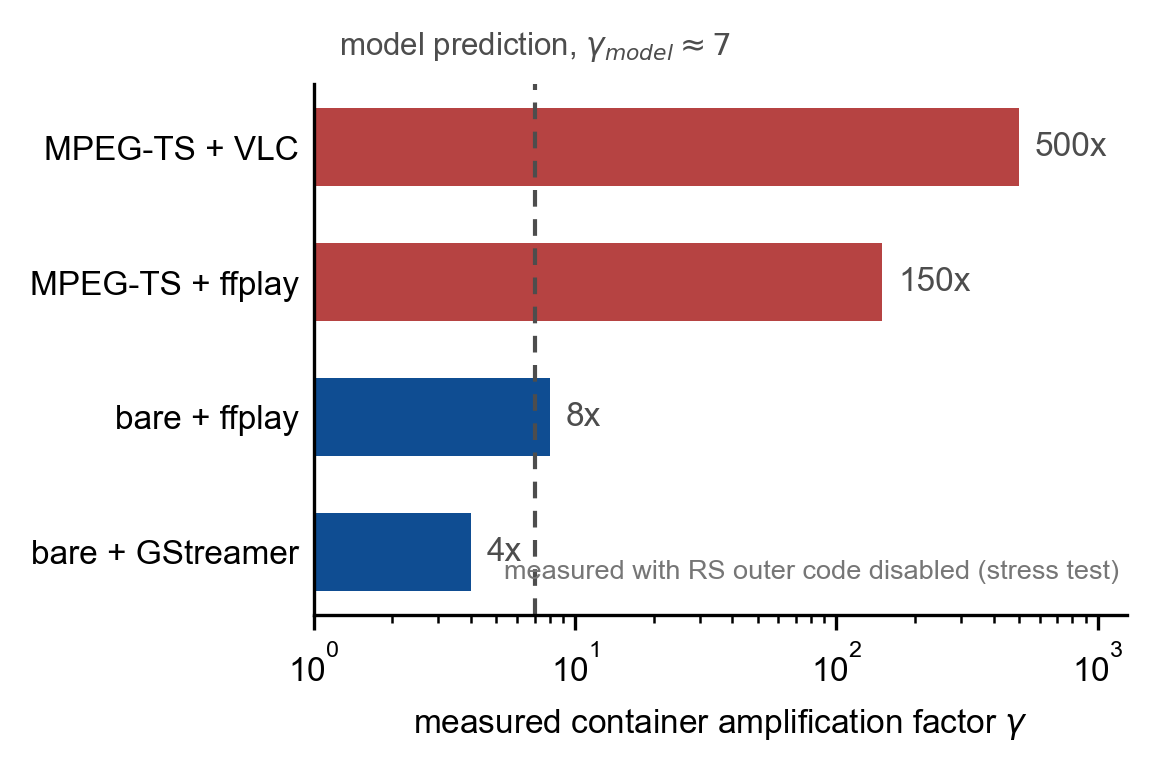
\includegraphics[width=\columnwidth]{fig3_gamma_mpl.png}
  \caption{Measured container amplification factor $\gamma$ for four transport stacks under the RS-disabled stress test (log scale). Dashed line: static header-exposure model prediction $\gamma_0 \approx 7$. MPEG-TS stacks (red) exceed the model prediction; bare-stream stacks (blue) fall below it.}
  \label{fig:gamma}
\end{figure}

Under this stress test (Table~\ref{tab:gamma} and Fig.~\ref{fig:gamma}): MPEG-TS + VLC produced 0\% usable playback (persistent frozen frames from PCR-clock deadlock); MPEG-TS + ffplay $\approx\!30\%$; bare H.264 + GStreamer $\approx\!95\%$, with the raw TS packet failure rate at 99.5\%.

The measured range ($4\times$--$500\times$) brackets the static header-exposure prediction ($7\times$): fault-tolerant decoders suppress the static exposure, while state-machine pathologies amplify it well above the static bound. The Markov-chain model correctly identifies the mechanism in both directions. With the outer code re-enabled, the same ordering persisted.

\subsection{Design Consequence}

On an ISAC link with a strong inner code and a minimal outer code, \textbf{MPEG-TS should be replaced by bare H.264 Annex~B}, and the decoder must be selected for fault tolerance (silent skip on damage, no PCR-clock coupling). GStreamer's \texttt{avdec\_h264} with \texttt{output-corrupt=true} meets both requirements.

% ─────────────────────────────────────────────────────────────────────────────
\section{Latency Optimization}
\label{sec:latency}

\subsection{Positive-Feedback Latency Loop}

The initial deployment used default queue depths of 32 frames at four pipeline stages (post-encode, post-modulate, pre-demodulate, synchronization). At 434\,frames/s, each queue contributes up to $\approx\!74$\,ms worst-case queuing delay. The interaction was not additive: when the H.264 decoder stalled, the UDP receive buffer filled, the demodulator's downstream send blocked, the LDPC decode thread back-pressured, and the synchronization queue grew further---a positive-feedback loop in which latency accumulated without bound.

The fix was structural: queue depths were reduced to the minimum sustaining continuous operation (16, 8, 4, 8 at the four stages respectively), and all blocking enqueues were replaced by \texttt{try\_push} semantics that drop on overflow. Drops convert unbounded latency growth into bounded, visible frame loss---the correct trade-off for a real-time service.

\subsection{Measured Latency}

End-to-end latency was measured by the stopwatch method (millisecond timer filmed simultaneously at camera and display; 30\,fps capture, $\approx\!33$\,ms resolution). After queue optimization, the five-minute trace shows $\mathbf{250.3 \pm 0.5\,\text{ms}}$ steady-state latency with no accumulation trend. Occasional deviations correspond to the decoder's internal reference-frame pool reset---a receiver software behavior, not a link effect.

\begin{table}[t]
  \centering
  \caption{End-to-End Latency Decomposition}
  \label{tab:latency}
  \begin{tabular}{lc}
    \toprule
    Component & Contribution (ms) \\
    \midrule
    H.264 decoder + GStreamer pipeline & $\approx\!200$ ($\sim\!80\%$) \\
    Buffering (all queues combined)    & $\approx\!27$ \\
    x264 encode                        & $\approx\!10$ \\
    FEC decode (RS + LDPC)             & $\approx\!5$ \\
    OFDM framing                       & 2.3 \\
    ISAC radio link                    & $\approx\!3$ \\
    Localhost UDP                      & $<5$ \\
    \midrule
    \textbf{Total}                     & $\approx\!\mathbf{250}$ \\
    \bottomrule
  \end{tabular}
\end{table}

\begin{figure*}[t]
  \centering
  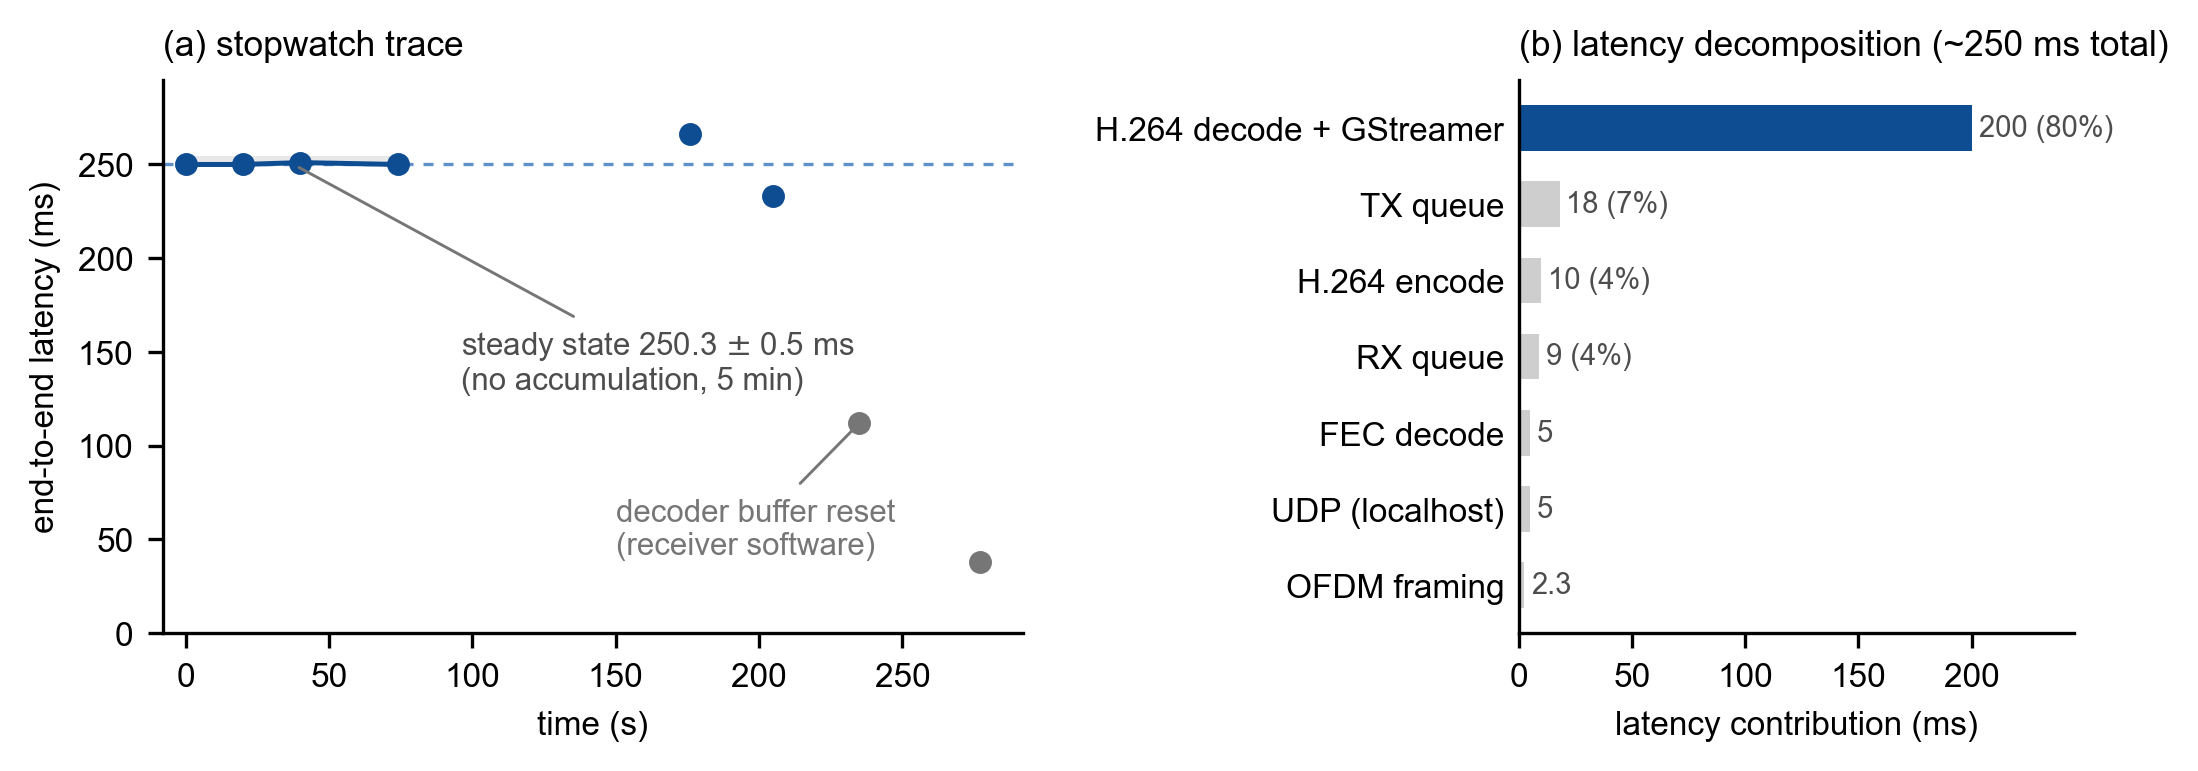
\includegraphics[width=\textwidth]{fig2_latency_mpl.png}
  \caption{End-to-end latency. (a)~Five-minute stopwatch trace; the shaded window marks the steady-state interval ($250.3 \pm 0.5$\,ms). Gray points are decoder-side buffer resets (receiver software, not the ISAC link). (b)~Latency decomposition: the H.264 decoder and GStreamer pipeline contribute $\approx\!80\%$ of the $\approx\!250$\,ms total; the ISAC radio contributes $\approx\!3$\,ms.}
  \label{fig:latency}
\end{figure*}

Table~\ref{tab:latency} and Fig.~\ref{fig:latency} show that the ISAC radio contributes $\approx\!3$\,ms. Further latency reduction on this platform requires targeting the decoder path, not the radio.

% ─────────────────────────────────────────────────────────────────────────────
\section{Discussion}
\label{sec:discussion}

\subsection{Least-Sufficient Protection}

The measurements above support a compact design principle for ISAC media services. \emph{Below} the container, protection is already more than sufficient: a $5\times10^{-10}$ LDPC residual means the outer code never fires in steady state, and the lightest configuration dominates on throughput. \emph{At and above} the container, protection is the scarcest resource: a default container choice multiplies effective failure exposure by $7\times$ (modeled) to $500\times$ (measured with an unforgiving decoder).

The engineering rule is therefore: \textbf{add protection where it is scarcest---container and decoder---and keep it minimal where residuals are already sparse---the outer FEC.} This is validated from both directions: with the outer code removed entirely, bare-stream + fault-tolerant decoder retained $\approx\!95\%$ usable playback while TS-based stacks failed completely.

\subsection{Boundary Conditions}

All results are bounded to: a single indoor line-of-sight link ($\approx\!5$\,m, QPSK, B210 receive platform), $640\times480$@20\,fps H.264, and one LDPC configuration (rate~1/2, 6~iterations). The $\gamma$ measurements derive from a disabled-outer-code stress regime; absolute $\gamma$ values are regime-specific, though the ordering is preserved in normal operation. The 16QAM modulation was compute-bound (CPU 105\% on B210) rather than channel-bound, identifying a platform ceiling rather than a waveform result. Future work includes adaptive outer-code switching driven by SNR, physical-layer-assisted error concealment, micro-Doppler sensing on the same waveform, and measured hardware upgrade results.

% ─────────────────────────────────────────────────────────────────────────────
\section{Conclusion}
\label{sec:conclusion}

On the OpenISAC platform carrying live H.264 video over the air, delivered video quality is decided above the channel code. The LDPC inner code's residual BER is below $5\times10^{-10}$, making the lightest Reed-Solomon outer code (14.3\% redundancy) both sufficient and Pareto-optimal, recovering 8.4\% payload throughput over the deployed heavier code. MPEG-TS encapsulation amplifies the same physical error stream by $7\times$ (Markov-chain model) to $500\times$ (measured worst-case decoder), and the amplification persists even when the outer code is active. Replacing MPEG-TS with bare H.264 Annex~B, selecting a fault-tolerant decoder, and shrinking queues to non-blocking minima yields $250\,\text{ms} \pm 0.5\,\text{ms}$ end-to-end latency---with the radio contributing $\approx\!3$\,ms---and zero-error payload delivery at $2.5\times$ video headroom. These results support a least-sufficient-protection design rule for ISAC media services: size the outer code to the measured residual, and reinvest the freed redundancy budget at the container and decoder layer.

\begin{figure}[t]
  \centering
  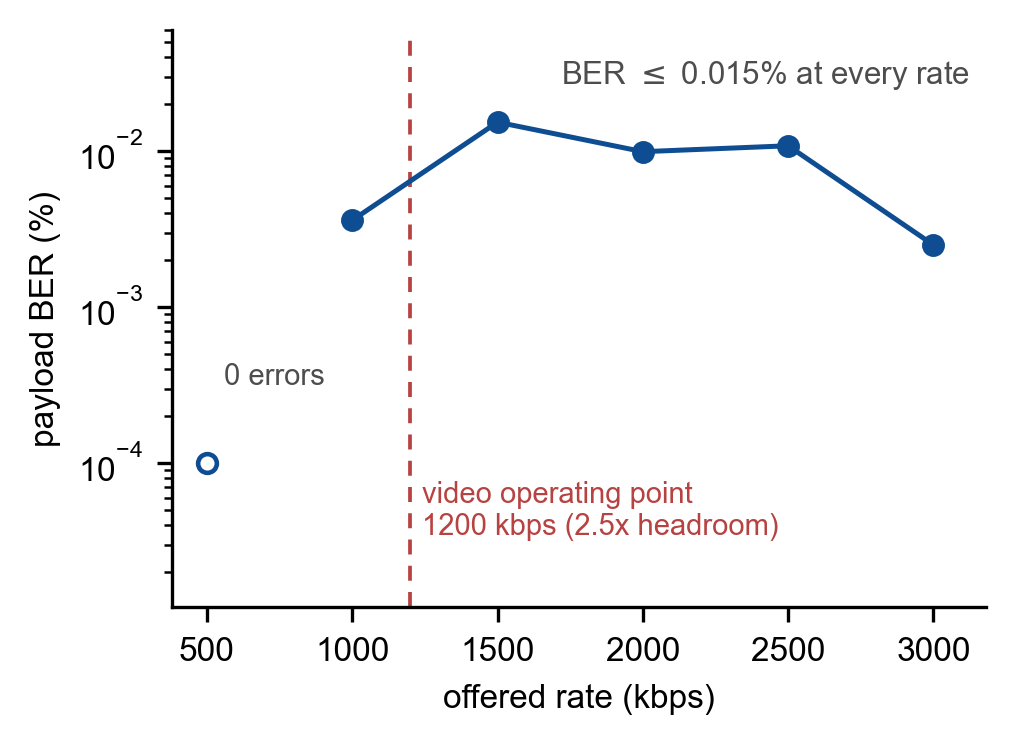
\includegraphics[width=\columnwidth]{fig5_ber_mpl.png}
  \caption{Payload BER versus offered rate under RS(255,223) protection. BER stays $\leq 0.015\%$ at every tested rate up to 3000\,kbps and is non-monotonic, consistent with pipeline occupancy rather than channel capacity. The dashed line marks the 1200\,kbps video operating point, which the link carries with $\approx\!2.5\times$ headroom. Open marker: zero errors at 500\,kbps.}
  \label{fig:ber}
\end{figure}

% ─────────────────────────────────────────────────────────────────────────────
\bibliographystyle{IEEEtran}
\begin{thebibliography}{9}

\bibitem{itu2023}
ITU-R, ``Framework and overall objectives of the future development of IMT for 2030 and beyond,''
Rec.\ ITU-R M.2160-0, Nov.\ 2023.

\bibitem{liu2022isac}
F.~Liu, Y.~Cui, C.~Masouros, J.~Xu, T.~X.~Han, Y.~C.~Eldar, and S.~Buzzi,
``Integrated sensing and communications: Toward dual-functional wireless networks for 6G and beyond,''
\emph{IEEE J.\ Sel.\ Areas Commun.}, vol.~40, no.~6, pp.~1728--1767, Jun.\ 2022.
doi:10.1109/JSAC.2022.3156632

\bibitem{wei2023survey}
Z.~Wei \emph{et al.},
``Integrated sensing and communication signals toward 5G-A and 6G: A survey,''
\emph{IEEE Internet Things J.}, early access, 2023.
arXiv:2301.03857.

\bibitem{zhou2026openisac}
Z.~Zhou, C.~Zhang, X.~Xu, and Y.~Zeng,
``OpenISAC: An open-source real-time experimentation platform for OFDM-ISAC with over-the-air synchronization,''
arXiv:2601.03535, Jan.\ 2026.

\bibitem{wiegand2003h264}
T.~Wiegand, G.~J.~Sullivan, G.~Bj{\o}ntegaard, and A.~Luthra,
``Overview of the H.264/AVC video coding standard,''
\emph{IEEE Trans.\ Circuits Syst.\ Video Technol.}, vol.~13, no.~7, pp.~560--576, Jul.\ 2003.
doi:10.1109/TCSVT.2003.815165

\bibitem{brunner2024bistatic}
D.~Brunner \emph{et al.},
``Bistatic OFDM-based ISAC with over-the-air synchronization: System concept and performance analysis,''
in \emph{Proc.\ IEEE ICC}, 2024.
arXiv:2405.04962.

\bibitem{cassagne2019aff3ct}
A.~Cassagne \emph{et al.},
``AFF3CT: A fast forward error correction toolbox!''
\emph{SoftwareX}, vol.~10, p.~100345, 2019.
doi:10.1016/j.softx.2019.100345

\bibitem{lin2004ecc}
S.~Lin and D.~J.~Costello,
\emph{Error Control Coding}, 2nd~ed.
Upper Saddle River, NJ: Prentice Hall, 2004.

\bibitem{iso13818}
ISO/IEC~13818-1:2022,
\emph{Information technology---Generic coding of moving pictures and associated audio information: Systems} (MPEG-TS), 2022.

\end{thebibliography}

\end{document}
